\documentclass{article}  
\usepackage[margin=1.0in]{geometry}            		% See geometry.pdf to learn the layout options. There are lots.
%\geometry{letterpaper}                   		% ... or a4paper or a5paper or ... 
%\usepackage[parfill]{parskip}    		% Activate to begin paragraphs with an empty line rather than an indent
\usepackage{graphicx}				% Use pdf, png, jpg, or eps§ with pdflatex; use eps in DVI mode
								% TeX will automatically convert eps --> pdf in pdflatex		
\usepackage{amsmath}
%\graphicspath{{/Users/lukebury/Documents/School/CU/ORCCA/}}
\usepackage{color}
\graphicspath{{../figures/}}

\newcommand{\paragraphtitle}[1]{\paragraph{#1}\mbox{}\\}

\title{Outline - APPM 5460 Proposal}
\author{Luke Bury \& Don Kuettel}

% Introduction

% History / Lit Review

% Application 

\begin{document}
\maketitle

% ==================================================================
% Introduction
\section{Introduction}
This proposal aims to investigate homoclinic orbits in the dynamical system known as the Circular Restricted Three-Body Problem (CR3PB). The CR3PB, further described in the following section, is a classical astrodynamics problem that has been studied for over 200 years and contains a plethora of interesting dynamical phenomena, including homoclinic orbits. 

In mathematics, a homoclinic orbit is defined as a trajectory of a flow of a dynamical system which joins a saddle equilibrium point to itself. More precisely, a homoclinic orbit lies in the intersection of the stable manifold, $W^s(p)$, and the unstable manifold, $W^u(p)$, of an equilibrium. Figure \ref{f:homoclinic_example} shows an example of a simple, two-dimensional homoclinic orbit about the saddle equilibrium point $p$. As the figure shows, as time approaches either negative or positive infinity, the homoclinic orbit will approach $p$. 

\begin{figure}[h!]
    \centering
    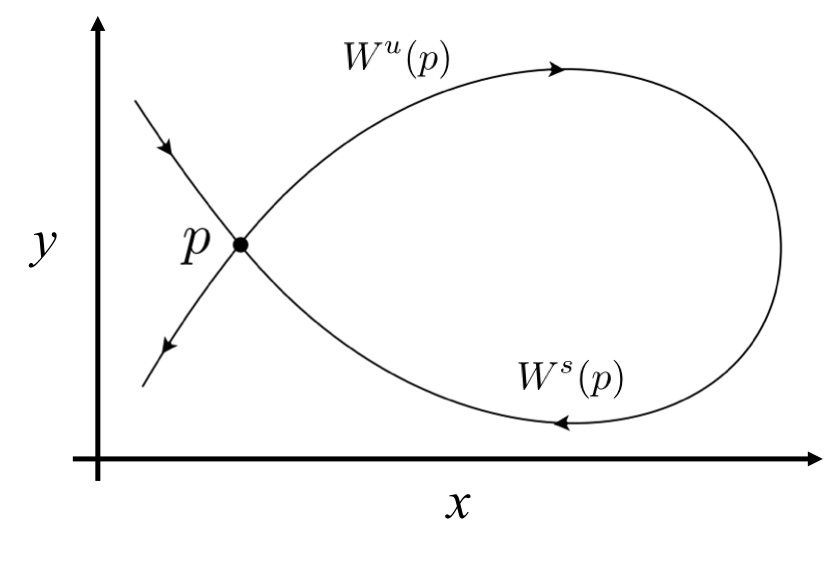
\includegraphics[width=4in]{homoclinic_orbit.png}
    \caption{This figure depicts a 2D homoclinic orbit.}
    \label{f:homoclinic_example}
\end{figure}

Homoclinic orbits, first discovered by Henri Poincar\'{e} in the 1885 Acta Mathematica competition sponsored by King Oscar II of Sweden, play an important role in the chaotic behavior of a dynamical system. Lying on the intersection between a stable and unstable manifold of the same equilibrium point, or orbit, the geometry of homoclinic orbits (i.e., the geometry of the manifold intersection) offers a way in which simple local information can be extrapolated to complicated global behavior. This proposal looks to study Poincar\'{e}'s work on homoclinic orbits and use that knowledge to find examples of homoclinic orbits in the CR3BP.
% ==================================================================


% ==================================================================
\bibliographystyle{plain}
\bibliography{../bibliography/appm5460.bib}
% ==================================================================

\end{document}  